\section{Results}
We demonstrated the performance of our algorithm using released influenza hemagglutinin
data set \philbs \ and a serum glycan data set \rphumanserum. Please refer to section
S\sref{S-sec:algorithm_performance} for all other datasets. For each comparison, the
unregularized case is not smoothed, effectively $\lambda = 0$, the partially regularized
case uses the grid search fitted values of $\mathbf{\tau}$ but uses a fixed $\lambda = 0.2$,
and the fully regularized case uses the grid search fitted values of both $\mathbf{\tau}$
and $\lambda$.

% begin variables collection from PhilBSStats.tex
\newcommand\PhilBSStatsCombinatorialGridROCAUC[0]{ 0.991\xspace}
\newcommand\PhilBSStatsCombinatorialGridTotal[0]{ 57\xspace}
\newcommand\PhilBSStatsCombinatorialPartialROCAUC[0]{ 0.995\xspace}
\newcommand\PhilBSStatsCombinatorialPartialTotal[0]{ 57\xspace}
\newcommand\PhilBSStatsCombinatorialUnregularizedROCAUC[0]{ 0.882\xspace}
\newcommand\PhilBSStatsCombinatorialUnregularizedTotal[0]{ 56\xspace}
\newcommand\PhilBSStatsGlyspaceGridROCAUC[0]{ 0.802\xspace}
\newcommand\PhilBSStatsGlyspaceGridTotal[0]{ 31\xspace}
\newcommand\PhilBSStatsGlyspacePartialROCAUC[0]{ 0.808\xspace}
\newcommand\PhilBSStatsGlyspacePartialTotal[0]{ 38\xspace}
\newcommand\PhilBSStatsGlyspaceUnregularizedROCAUC[0]{ 0.811\xspace}
\newcommand\PhilBSStatsGlyspaceUnregularizedTotal[0]{ 40\xspace}
\newcommand\PhilBSStatsKrambeckGridROCAUC[0]{ 0.742\xspace}
\newcommand\PhilBSStatsKrambeckGridTotal[0]{ 29\xspace}
\newcommand\PhilBSStatsKrambeckPartialROCAUC[0]{ 0.742\xspace}
\newcommand\PhilBSStatsKrambeckPartialTotal[0]{ 29\xspace}
\newcommand\PhilBSStatsKrambeckUnregularizedROCAUC[0]{ 0.742\xspace}
\newcommand\PhilBSStatsKrambeckUnregularizedTotal[0]{ 28\xspace}


% begin variables collection from Serum.tex
\newcommand\SerumCombinatorialGridROCAUC[0]{ 0.804\xspace}
\newcommand\SerumCombinatorialGridTotal[0]{ 86\xspace}
\newcommand\SerumCombinatorialGridTotalSimplified[0]{ 61\xspace}
\newcommand\SerumCombinatorialPartialROCAUC[0]{ 0.816\xspace}
\newcommand\SerumCombinatorialPartialTotal[0]{ 87\xspace}
\newcommand\SerumCombinatorialPartialTotalSimplified[0]{ 62\xspace}
\newcommand\SerumCombinatorialUnregularizedROCAUC[0]{ 0.679\xspace}
\newcommand\SerumCombinatorialUnregularizedTotal[0]{ 86\xspace}
\newcommand\SerumCombinatorialUnregularizedTotalSimplified[0]{ 61\xspace}
\newcommand\SerumGlyspaceGridROCAUC[0]{ 0.809\xspace}
\newcommand\SerumGlyspaceGridTotal[0]{ 60\xspace}
\newcommand\SerumGlyspaceGridTotalSimplified[0]{ 52\xspace}
\newcommand\SerumGlyspacePartialROCAUC[0]{ 0.803\xspace}
\newcommand\SerumGlyspacePartialTotal[0]{ 60\xspace}
\newcommand\SerumGlyspacePartialTotalSimplified[0]{ 52\xspace}
\newcommand\SerumGlyspaceUnregularizedROCAUC[0]{ 0.788\xspace}
\newcommand\SerumGlyspaceUnregularizedTotal[0]{ 59\xspace}
\newcommand\SerumGlyspaceUnregularizedTotalSimplified[0]{ 51\xspace}
\newcommand\SerumKrambeckGridROCAUC[0]{ 0.882\xspace}
\newcommand\SerumKrambeckGridTotal[0]{ 69\xspace}
\newcommand\SerumKrambeckGridTotalSimplified[0]{ 59\xspace}
\newcommand\SerumKrambeckPartialROCAUC[0]{ 0.883\xspace}
\newcommand\SerumKrambeckPartialTotal[0]{ 70\xspace}
\newcommand\SerumKrambeckPartialTotalSimplified[0]{ 60\xspace}
\newcommand\SerumKrambeckUnregularizedROCAUC[0]{ 0.866\xspace}
\newcommand\SerumKrambeckUnregularizedTotal[0]{ 70\xspace}
\newcommand\SerumKrambeckUnregularizedTotalSimplified[0]{ 60\xspace}



\subsection{Chromatogram Assignment Performance for \philbs}
    The fitted parameters for the network constructed for \philbs are shown in
    Table~\ref{tab:parameter_estimates}. The assigned chromatograms are shown in
    Figure~\ref{fig:philbs_assignments}. We observe up to seven branch structures in
    this sample, consistent with these \nglycans being derived from an avian context
    (\cite{Stanley2009,Khatri2016a}).

    \begin{table}[tb]
        \tiny
        \begin{tabular}{l SSSSSS}
            \toprule
            \multirow{3}{*}{Neighborhood $\tau$} &
                \multicolumn{3}{c}{Phil-BS} &
                \multicolumn{3}{c}{Serum} \\
                & {Combinatorial +} & {\glyspace} & {Krambeck} & {Combinatorial} & {\glyspace} & {Krambeck}\\
                & {Sulfate}                 &             &            &                 &             & \\
            \midrule
            high-mannose           & 18.008 & 15.061 & 17.089 & 20.328 & 19.392 & 19.720\\
            hybrid                 & 13.440 & 12.435 & 12.503 & 20.997 & 18.610 & 20.056\\
            bi-antennary           & 0.000  & 0.000  & 0.000  & 15.901 & 16.826 & 17.593\\
            asialo-bi-antennary    & 14.078 & 10.916 & 13.591 & 22.585 & 21.563 & 21.827\\
            tri-antennary          & 0.000  & 0.000  & 0.000  & 26.420 & 19.605 & 23.644\\
            asialo-tri-antennary   & 14.538 & 6.565  & 11.952 & 20.025 & 21.128 & 19.764\\
            tetra-antennary        & 0.000  & 0.000  & 0.000  & 19.508 & 18.542 & 17.674\\
            asialo-tetra-antennary & 14.331 & 4.842  & 12.373 & 2.472  & 7.180  & 2.568\\
            penta-antennary        & 0.000  & 0.000  & 0.000  & 11.878 & 15.035 & 11.682\\
            asialo-penta-antennary & 11.588 & 1.255  & 9.784  & 0.000  & 0.000  & 0.000\\
            hexa-antennary         & 0.000  & 0.000  & 0.000  & 0.000  & 0.000  & 0.000\\
            asialo-hexa-antennary  & 11.094 & 3.883  & 13.223 & 0.000  & 0.000  & 0.000\\
            hepta-antennary        & 0.000  & 0.000  & 0.000  & 0.000  & 0.000  & 0.000\\
            asialo-hepta-antennary & 3.117  & 1.529  & 2.703  & 0.000  & 0.000  & 0.000\\
            \midrule
            ${\hat \lambda}$       & 0.99   & 0.69   & 0.99   & 0.99   & 0.99   & 0.99\\
            ${\hat \gamma}$        & 11.39  & 14.60  & 10.42  & 20.57  & 18.42  & 20.72\\
            \bottomrule
        \end{tabular}
        \caption{Estimated values of smoothing parameters $\tau$, $\lambda$, and $\gamma$ for each
                 dataset and database\label{tab:parameter_estimates}}
    \end{table}
    \hfill
    \begin{figure}[tb]
        \caption{Chromatogram Assignments and Quantification
                 for \philbs Using the \textit{Combinatorial + Sulfate} database.
                 \label{fig:philbs_assignments}. The Retention Time (Min) axis shows
                 the retention time in minutes from the experiment, and the Relative
                 Abundance axis shows the intensity of the signal from the particular
                 aggregated ion species for each analyte. The identified glycan compositions
                 are labeled with a tuple describing the number of each component of the form
                 [\monosaccharide{HexNAc}, \monosaccharide{Hex}, \monosaccharide{Fuc},
                  \monosaccharide{NeuAc}, \monosaccharide{SO3}]}
        \centering
        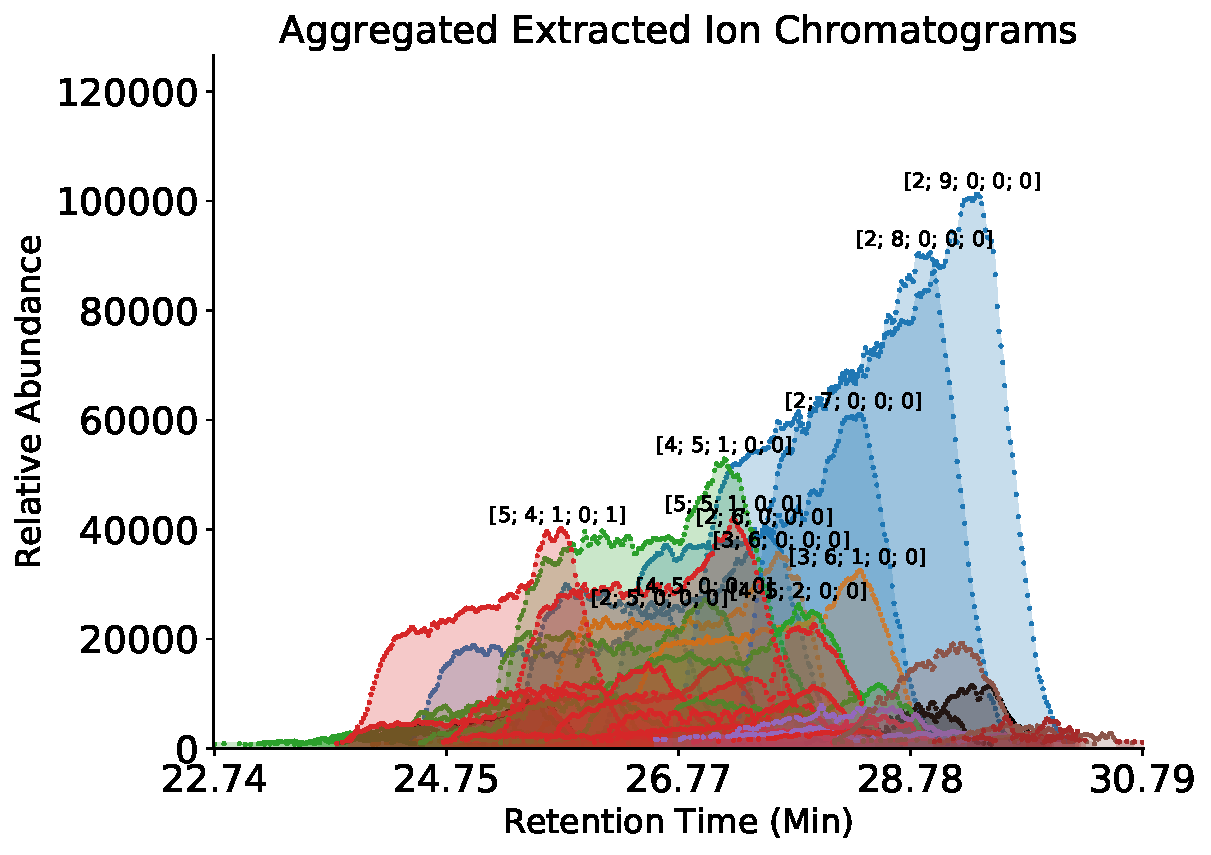
\includegraphics[width=0.45\textwidth,valign=t]{figure/sulfated_phil_bs_native_chromatograms.pdf}
        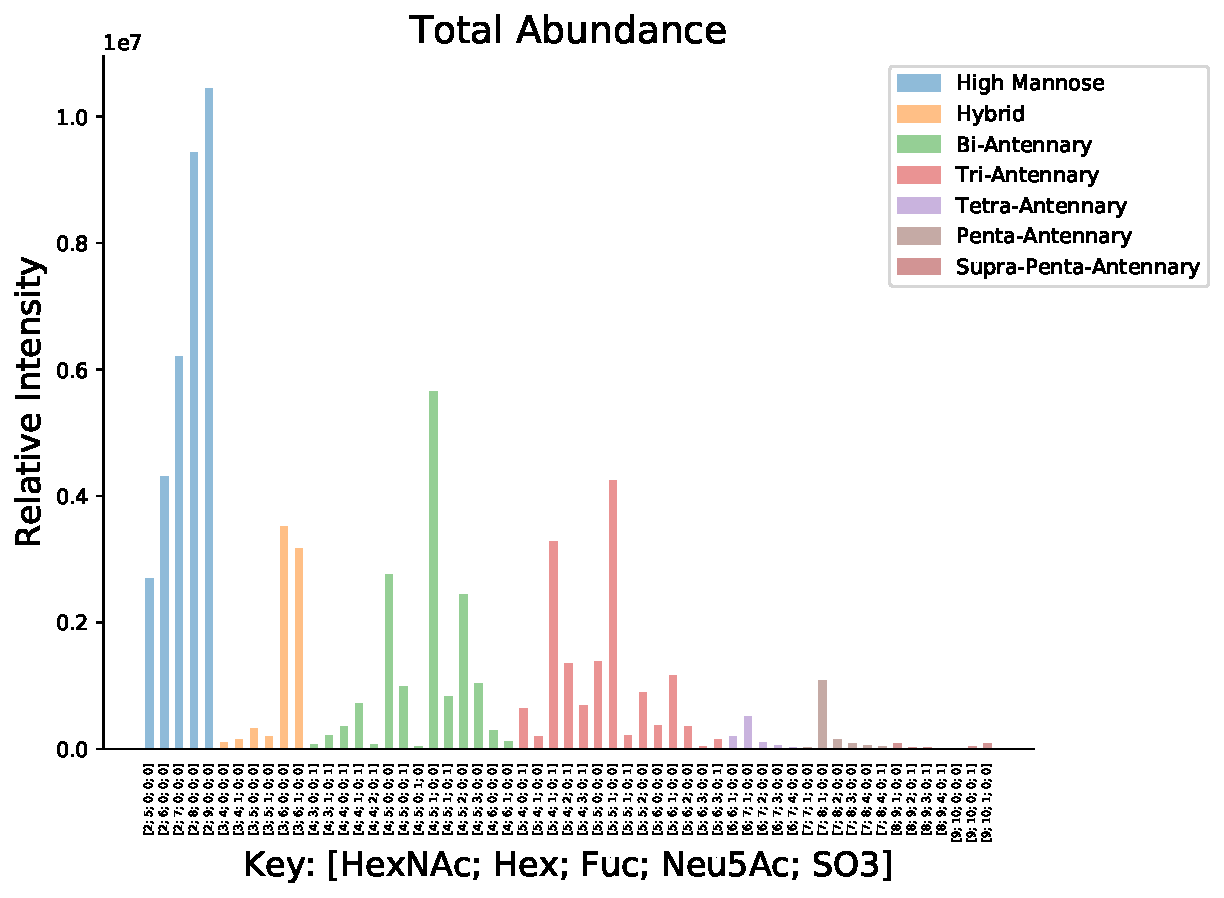
\includegraphics[width=0.45\textwidth,valign=t]{figure/sulfated_phil_bs_native_abundances.pdf}
    \end{figure}
    \hfill
    \begin{figure}[htb]
        \caption{Performance Comparison with and without Network Smoothing for \philbs
                 \label{fig:philbs_perf}. The Receiver Operator Characteristic Curve (ROC)
                 comparing True Positive Rate (TPR) to False Positive Rate (FPR) shows how
                 each database performed under different regularization conditions, summarized
                 with the Area Under the Curve (AUC) in the legend. The \textit{Combinatorial + Sulfate}
                 database showed the best performance, and improved with regularization.}
        \centering
        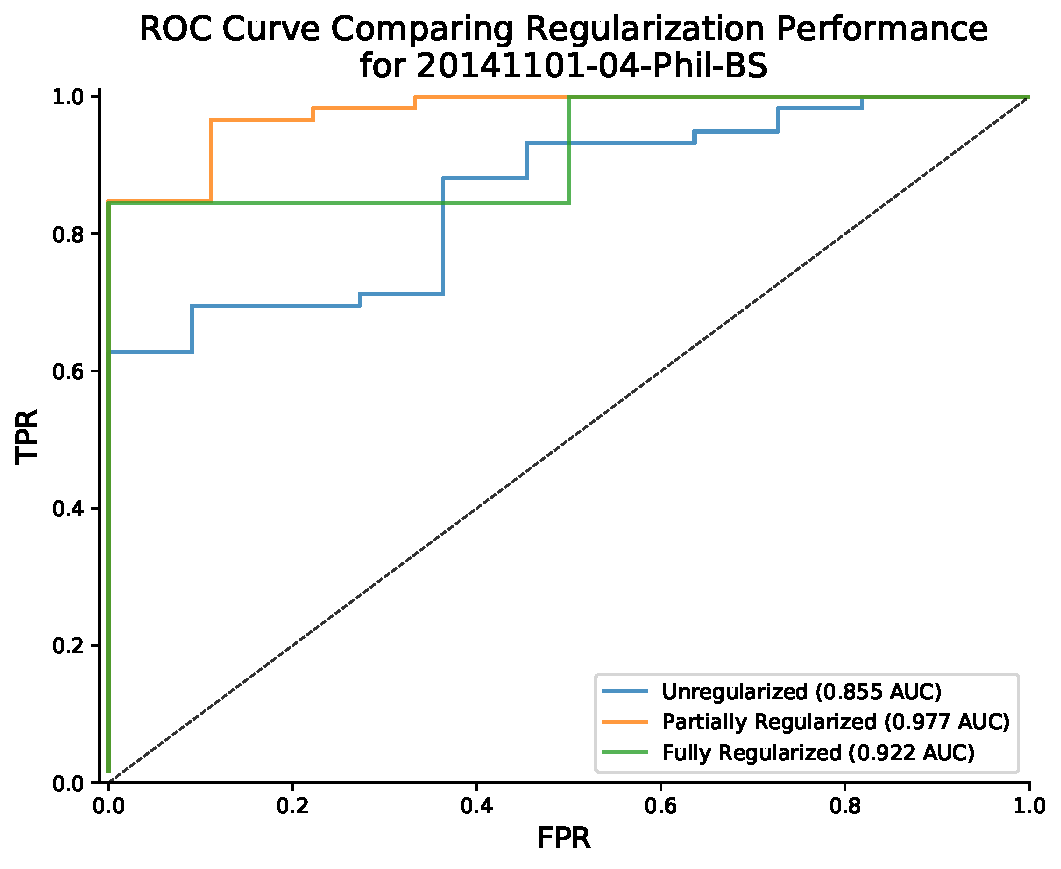
\includegraphics[width=0.45\textwidth,valign=t]{figure/sulfated_phil_bs_native_roc.pdf}
        % 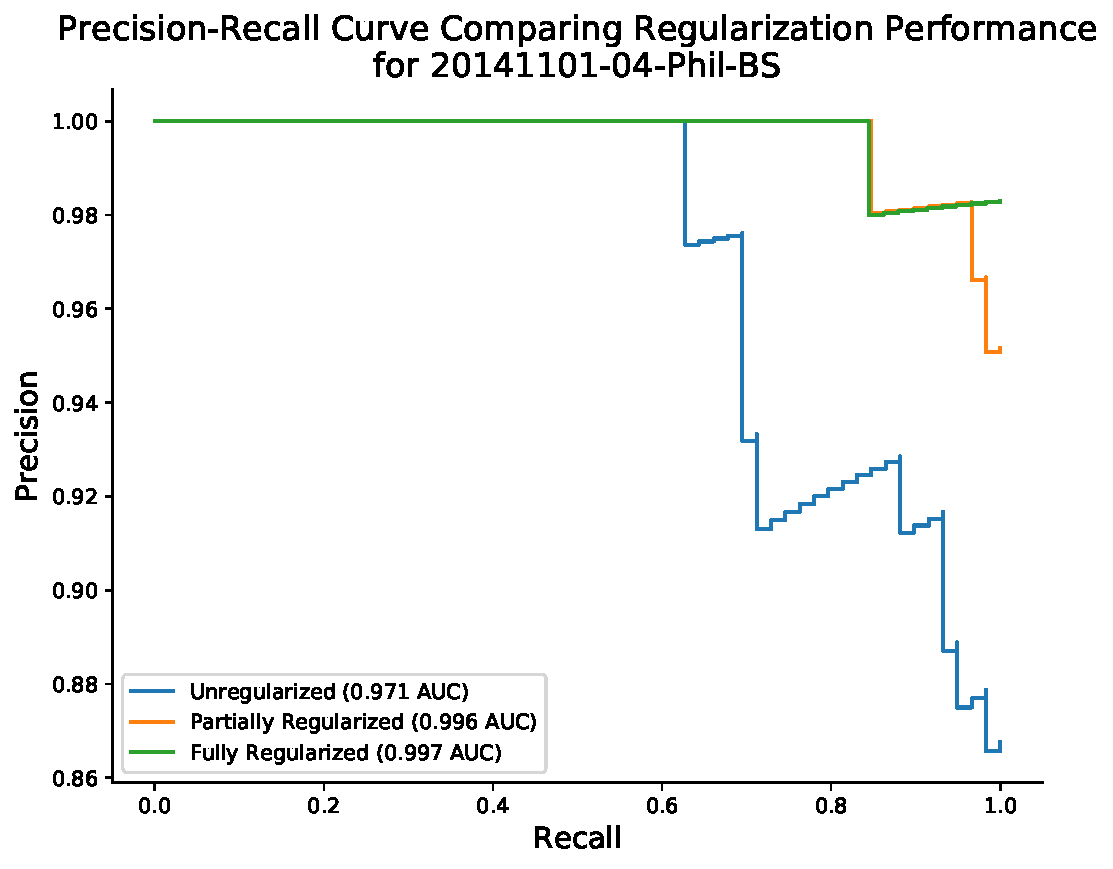
\includegraphics[width=0.45\textwidth,valign=t]{figure/sulfated_phil_bs_native_prec_rec.pdf}
    \end{figure}

    The comparison of assignment performance with differing degrees of smoothing for each database
    are shown in Figure~\ref{fig:philbs_perf} and Table \ref{tab:philbs_statistics}. \reviewchange{We used
    the Receiver Operator Characteristic (ROC) Area Under the Curver (AUC) to measure performance,
    using manually validated compositions as ground truth}. We observed the greatest number of
    assignments using the \textit{Combinatorial + Sulfate} database, and the greatest ROC AUC in
    the partially regularized condition.

    \begin{table}[!htb]
        \scriptsize
        \centering
        \begin{threeparttable}
            \begin{tabular}{p{4.1cm} S c}
                \toprule
                Name & ROC\ AUC & True Matches\tnote{1} \\
                     % & AUC & Matches\\
                \midrule
                Combinatorial Unregularized & \PhilBSStatsCombinatorialUnregularizedROCAUC &
                                              \PhilBSStatsCombinatorialUnregularizedTotal \\
                Combinatorial Partial       & \PhilBSStatsCombinatorialPartialROCAUC &
                                              \PhilBSStatsCombinatorialPartialTotal \\
                Combinatorial Grid          & \PhilBSStatsCombinatorialGridROCAUC &
                                              \PhilBSStatsCombinatorialGridTotal \\
                GlySpace Unregularized      & \PhilBSStatsGlyspaceUnregularizedROCAUC &
                                              \PhilBSStatsGlyspaceUnregularizedTotal \\
                GlySpace Partial            & \PhilBSStatsGlyspacePartialROCAUC &
                                              \PhilBSStatsGlyspacePartialTotal \\
                GlySpace Grid               & \PhilBSStatsGlyspaceGridROCAUC &
                                              \PhilBSStatsGlyspaceGridTotal \\
                Krambeck Unregularized      & \PhilBSStatsKrambeckUnregularizedROCAUC &
                                              \PhilBSStatsKrambeckUnregularizedTotal \\
                Krambeck Partial            & \PhilBSStatsKrambeckPartialROCAUC &
                                              \PhilBSStatsKrambeckPartialTotal \\
                Krambeck Grid               & \PhilBSStatsKrambeckGridROCAUC &
                                              \PhilBSStatsKrambeckGridTotal \\
                \cite{Khatri2016a} & {-} & 46 \\
                \bottomrule
            \end{tabular}
            \begin{tablenotes}
                \item[1] Selected at $\phi_o > 5.0$
            \end{tablenotes}
            \captionof{table}{Performance Comparison for \philbs\label{tab:philbs_statistics}, using
            \reviewchange{Receiver Operator Characteristic (ROC) Area Under the Curver (AUC)}. The Combinatorial Partial
            Regularization approach performed best.}
        \end{threeparttable}
    \end{table}

\subsection{Chromatogram Assignment Performance for \rpserum}
    The fitted parameters for the network constructed for \rpserum are shown in
    Table~\ref{tab:parameter_estimates}. The assigned chromatograms are shown in
    Figure~\ref{fig:rpserum_assignments}.

    \begin{figure}[htb]
        \caption{Performance Comparison with and without Network Smoothing for \rpserum
                 \label{fig:rpserum_perf}. The Receiver Operator Characteristic Curve (ROC)
                 comparing True Positive Rate (TPR) to False Positive Rate (FPR) shows how
                 each database performed under different regularization conditions, summarized
                 with the Area Under the Curve (AUC) in the legend}
        \centering
        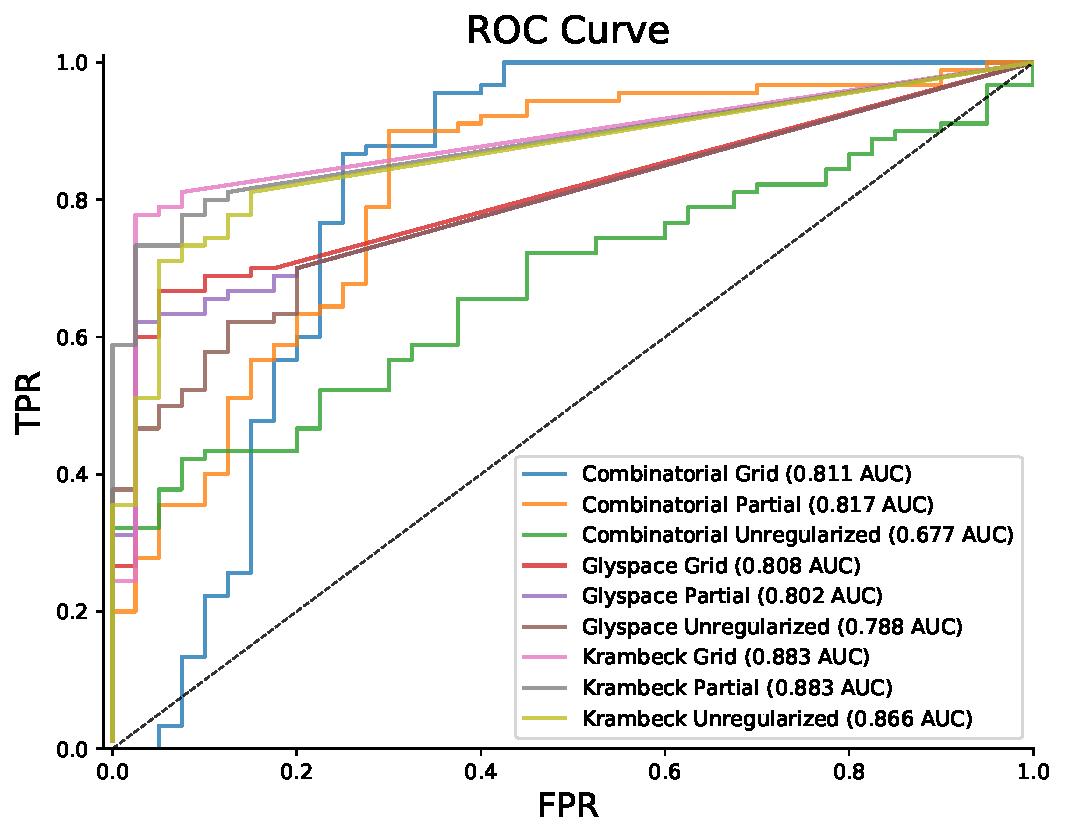
\includegraphics[width=0.45\textwidth,valign=t]{figure/serum_roc.pdf}
        % 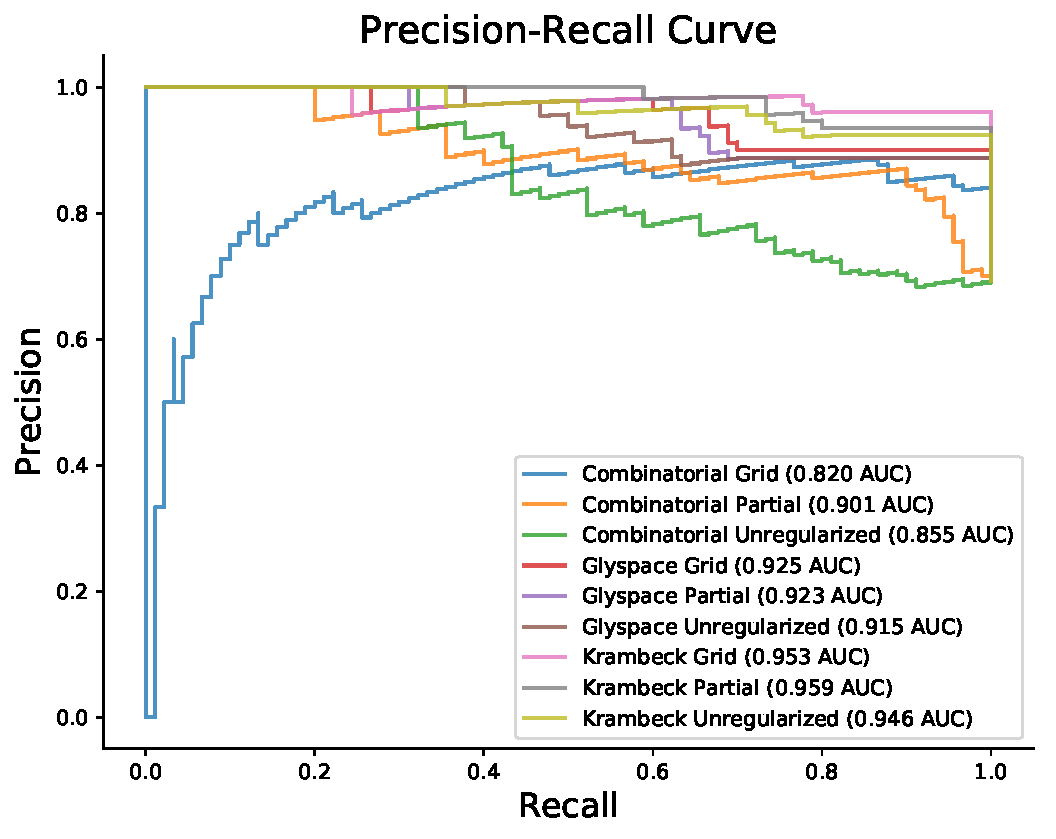
\includegraphics[width=0.45\textwidth,valign=t]{figure/serum_prec_rec.pdf}
    \end{figure}

    \begin{figure}[tb]
        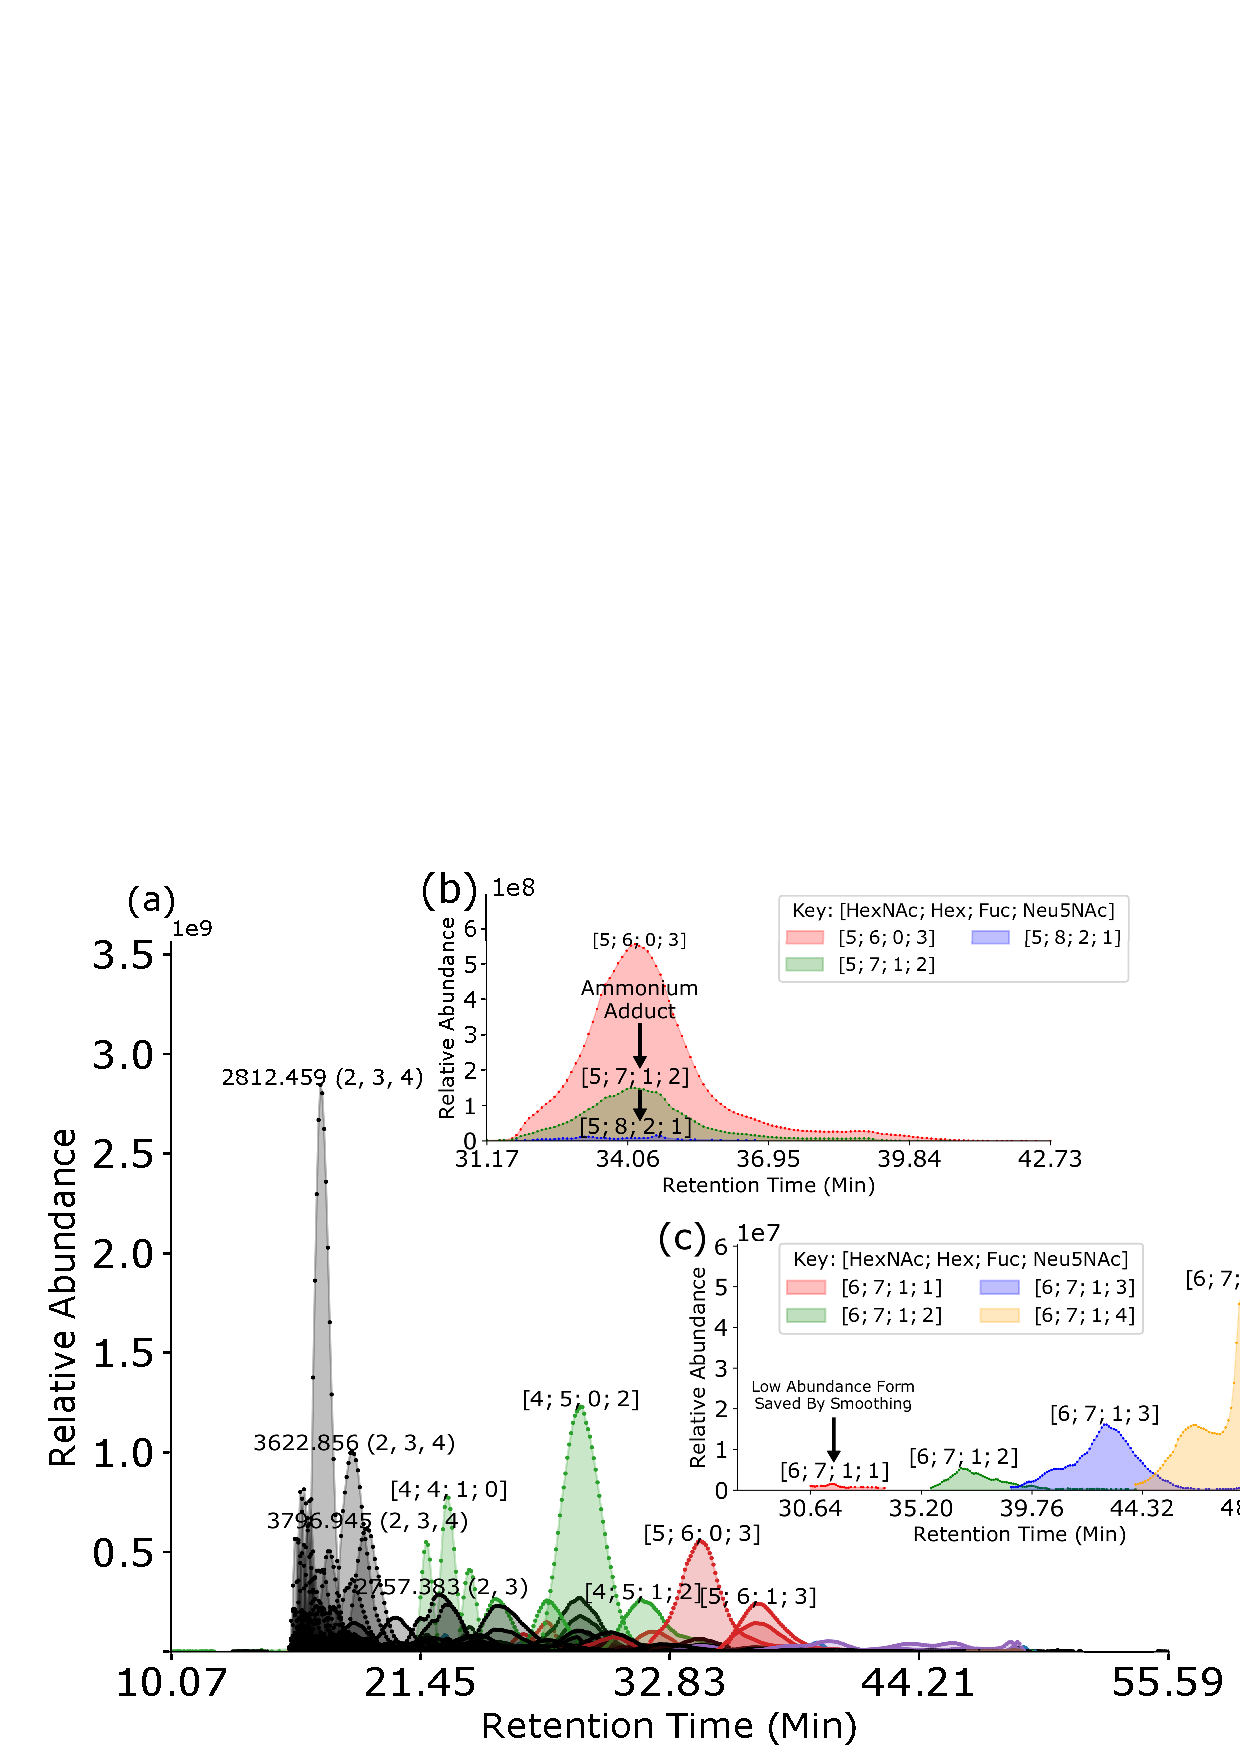
\includegraphics[width=0.5\textwidth, valign=t]{figure/rp_serum_chromatogram_details.pdf}
        \caption{Chromatogram Assignments for \rpserum. In all panels, the Retention Time (Min) axis shows
            the retention time in minutes from the experiment, and the Relative
            Abundance axis shows the intensity of the signal from the particular
            aggregated ion species for each analyte. The identified glycan compositions
            are labeled with a tuple describing the number of each component of the form
            [\monosaccharide{HexNAc}, \monosaccharide{Hex}, \monosaccharide{Fuc}, \monosaccharide{NeuAc}]
            (a) Features Assigned After Grid Regularization of \rpserum (b) Low scoring features
            which may be discarded based on individual evidence alone may be more reasonable to accept
            given evidence from related composition, such as our network smoothing method (c) This sample
            contains heavy ammonium adduction which introduces ambiguity in intact mass based assignments
            \label{fig:rpserum_assignments}
        }
    \end{figure}

    \begin{table}[!htb]
        \scriptsize
        \begin{threeparttable}
            \begin{tabular}{p{3cm} S c c}
                \toprule
                Name & ROC AUC & True Matches\tnote{1} & Non-Ambiguous Matches\\
                \midrule
                Combinatorial Unregularized & \SerumCombinatorialUnregularizedROCAUC &
                                              \SerumCombinatorialUnregularizedTotal &
                                              \SerumCombinatorialUnregularizedTotalSimplified \\
                Combinatorial Partial       & \SerumCombinatorialPartialROCAUC &
                                              \SerumCombinatorialPartialTotal &
                                              \SerumCombinatorialPartialTotalSimplified \\
                Combinatorial Grid          & \SerumCombinatorialGridROCAUC &
                                              \SerumCombinatorialGridTotal &
                                              \SerumCombinatorialGridTotalSimplified \\
                GlySpace Unregularized      & \SerumGlyspaceUnregularizedROCAUC &
                                              \SerumGlyspaceUnregularizedTotal &
                                              \SerumGlyspaceUnregularizedTotalSimplified \\
                GlySpace Partial            & \SerumGlyspacePartialROCAUC &
                                              \SerumGlyspacePartialTotal &
                                              \SerumGlyspacePartialTotalSimplified \\
                GlySpace Grid               & \SerumGlyspaceGridROCAUC &
                                              \SerumGlyspaceGridTotal &
                                              \SerumGlyspaceGridTotalSimplified \\
                Krambeck Unregularized      & \SerumKrambeckUnregularizedROCAUC &
                                              \SerumKrambeckUnregularizedTotal &
                                              \SerumKrambeckUnregularizedTotalSimplified \\
                Krambeck Partial            & \SerumKrambeckPartialROCAUC &
                                              \SerumKrambeckPartialTotal &
                                              \SerumKrambeckPartialTotalSimplified \\
                Krambeck Grid               & \SerumKrambeckGridROCAUC &
                                              \SerumKrambeckGridTotal &
                                              \SerumKrambeckGridTotalSimplified \\
                \cite{Yu2013}               & {-} & 72\tnote{2} & 59 \\
                \bottomrule
            \end{tabular}
            \begin{tablenotes}
                \item[1] Selected at $\phi_o > 5.0$
                \item[2] Only includes cases with sufficient MS1 scans available
                         for comparison
            \end{tablenotes}
        \end{threeparttable}
        \captionof{table}{Performance Comparison for \rpserum\label{tab:serum_statistics}, using
            \reviewchange{Receiver Operator Characteristic (ROC) Area Under the Curver (AUC)} and number of non-ambiguous
            matches. While the Krambeck database had a better ROC AUC, the Combinatorial database had more
            true matches.}
    \end{table}

    The comparison of assignment performance with differing degrees of smoothing is
    shown in Figure~\ref{fig:rpserum_perf}. We observe the greatest number of total true
    identifications using the partially regularized Combinatorial database. However, the
    Combinatorial database also has many more false positives, with a ROC AUC of \SerumCombinatorialPartialROCAUC.
    These false positives do not appear in the biosynthetically constraind Krambeck database
    which maximizes its ROC AUC in the partially regularized condition at \SerumKrambeckPartialROCAUC.
    After removing all ambiguous matches, the Krambeck database also has nearly the same
    number of true matches as the Combinatorial database.
